\documentclass[12pt,a4paper]{article}

% Margins.
\setlength{\oddsidemargin}{0in}
\setlength{\evensidemargin}{0in}
\setlength{\headheight}{12pt}
\setlength{\headsep}{42pt}
\setlength{\topmargin}{-54pt}
\setlength{\textwidth}{6.5in}
\setlength{\textheight}{10in}

\usepackage{amsmath}
\usepackage{float}
\usepackage{graphicx}
\usepackage[hyphens]{url}
\usepackage{hyperref}	% Clickable links to figures, references and urls.
\usepackage{datetime}
\usepackage{longtable}

% Links direct to top of figures.
\usepackage[all]{hypcap}

% Drawing.
\usepackage{pgf}
\usepackage{tikz}

% Listings for formatting code.
\usepackage{listings}
\usepackage{textcomp}
% General options.
\lstset{breaklines=true, basicstyle=\small\ttfamily, tabsize=4, numbers=left, stepnumber=1, frame=single, showstringspaces=false, upquote=true}
% C++ specific high-lighting. Comments are 50/50 shades of green/black and strings coloured with 60/40 red/black mixture.
\lstset{language=[ISO]C++, commentstyle=\color{green!50!black}, keywordstyle=\color{blue}, stringstyle=\color{red!60!black}}

%opening
\title{\vspace{-2cm}Physics for Engineers\\Class 08\\Differential Length, Surface and Volume Elements}
\author{Attique Dawood}
\date{February 10, 2013\\[0.2cm] Last Modified: \today, \currenttime}
\begin{document}
\maketitle
\section{Announcements}
\begin{itemize}
\item None.
\end{itemize}
\section{Revision}
\begin{itemize}
\item Constant coordinate surfaces in Cartesian, cylindrical and spherical coordinate systems.
\end{itemize}
\section{Differential Length, Surface and Volume Elements (3.2S)}
\subsection{Differential Length, Surface and Volume in Cartesian Coordinates}
In Cartesian coordinates a differential length element is generalised displacement in 3D space. Differential length is a vector. It is defined as,
\begin{equation}
d\textbf{\textit{l}}=dx\hat x+dy\hat y+dz\hat z
\end{equation}
The differential surface elements corresponding to $x=constant$, $y=constant$ and $z=constant$ planes are
\begin{equation}
\begin{split}
d\textbf{A}~\mathrm{or}~d\textbf{S}=~&dydz\hat x\\
&dxdz\hat y\\
&dxdy\hat z.
\end{split}
\end{equation}
The differential volume element is
\begin{equation}
dv=dxdydz
\end{equation}
\begin{figure}[H]
\centering
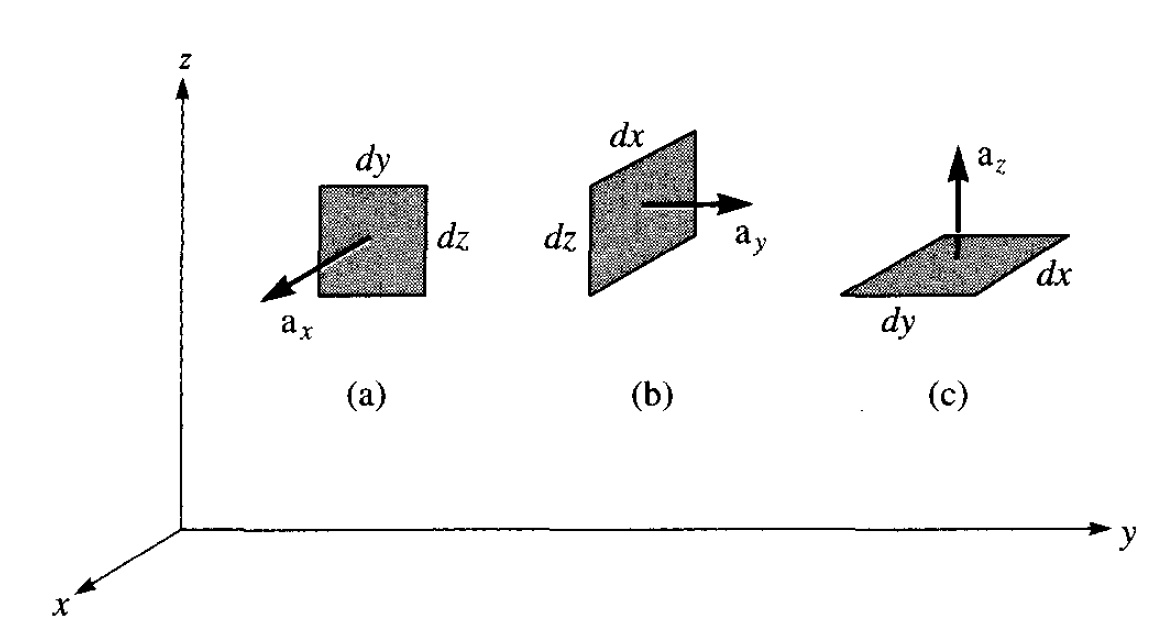
\includegraphics[scale=0.3]{Figure3-2S.png}
\caption{Differential normal areas in Cartesian coordinates. Figure taken from~\cite[Figure 3.2, page 54]{Sadiku}}
\label{Cartesian-differential-area}
\end{figure}
\subsection{Differential Length, Surface and Volume in Cylindrical Coordinates}
In Cylindrical coordinates differential length is defined as,
\begin{equation}
d\textbf{\textit{l}}=d\rho\hat \rho+\rho d\phi\hat \phi+dz\hat z
\end{equation}
Note that $d\phi$ is only an angle. Corresponding to a change in angle $d\phi$ the differential displacement/length is the arc length $\rho d\phi$. The differential surface elements corresponding to $\rho=constant$, $\phi=constant$ and $z=constant$ planes are
\begin{equation}
\begin{split}
d\textbf{A}~\mathrm{or}~d\textbf{S}=~&\rho d\phi dz\hat \rho\\
&d\rho dz\hat \phi\\
&\rho d\rho d\phi\hat z.
\end{split}
\end{equation}
The differential volume element is
\begin{equation}
dv=\rho d\rho d\phi dz
\end{equation}
\begin{figure}[htb]
\centering
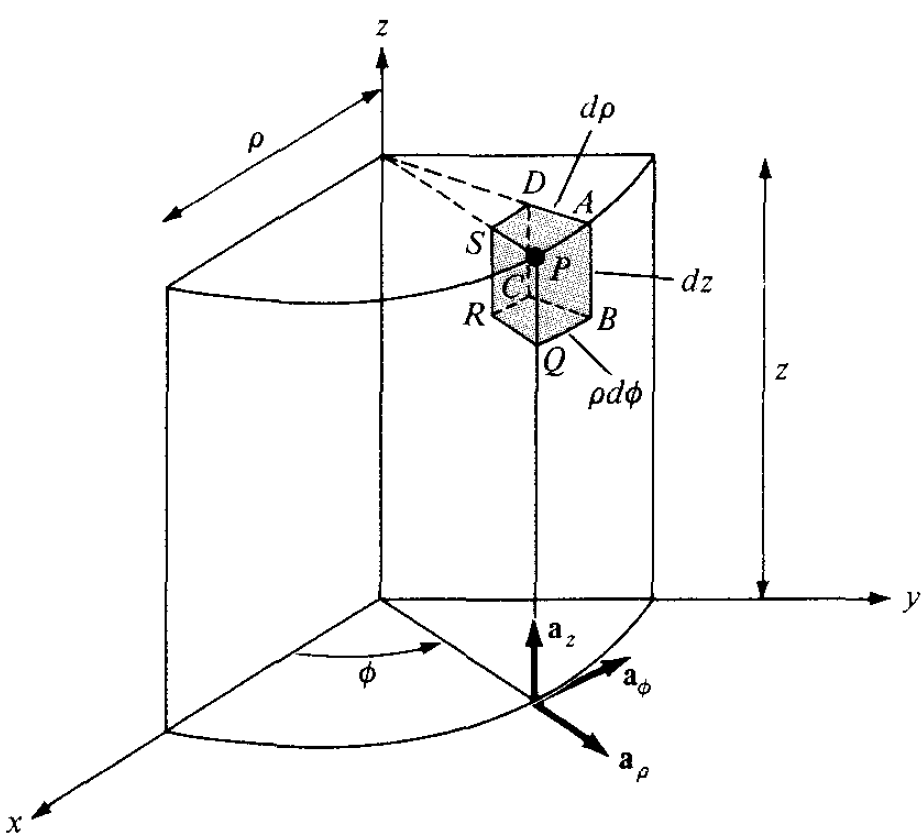
\includegraphics[scale=0.3]{Figure3-3S.png}
\caption{Differential volume in Cylindrical coordinates. Figure taken from~\cite[Figure 3.3, page 56]{Sadiku}}
\label{Cylindrical-differential-volume}
\end{figure}
\begin{figure}[htb]
\centering
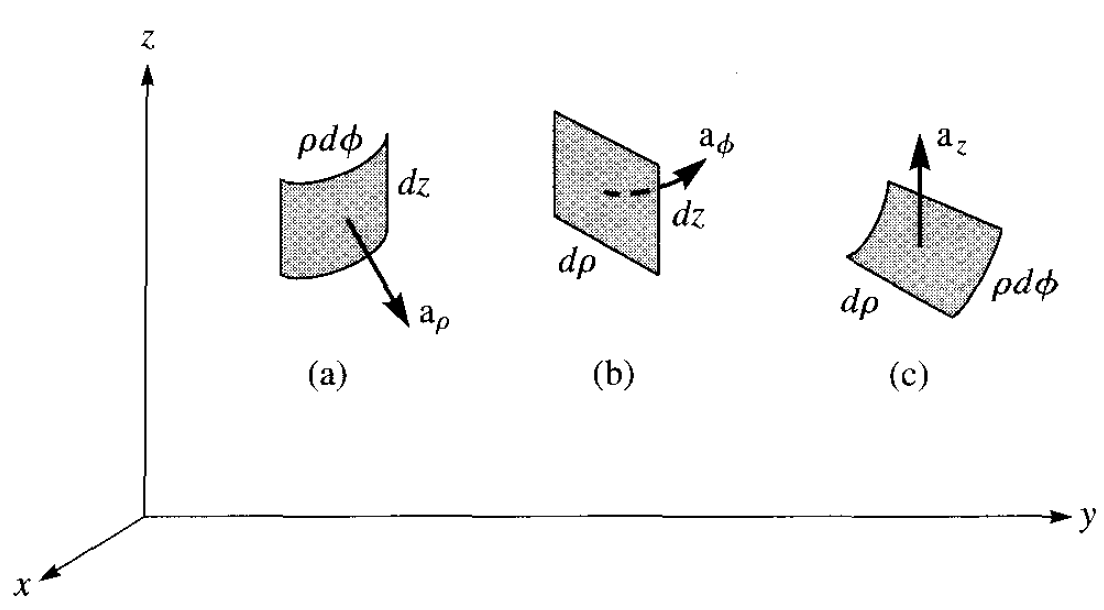
\includegraphics[scale=0.3]{Figure3-4S.png}
\caption{Differential normal areas in Cylindrical coordinates. Figure taken from~\cite[Figure 3.4, page 56]{Sadiku}}
\label{Cylindrical-differential-area}
\end{figure}
\subsection{Differential Length, Surface and Volume in Spherical Coordinates}
In Spherical coordinates differential length is defined as,
\begin{equation}
d\textbf{\textit{l}}=dr\hat r+r d\theta\hat \theta+r\sin\theta d\phi\hat \phi
\end{equation}
Note that $d\theta$ and $d\phi$ are angles. Corresponding to change in angles $d\theta$ and $d\phi$ the differential displacements are the arc lengths $rd\theta$ and $r\sin\theta d\phi$. Note that $\rho=r\sin\theta$ in Spherical coordinates. The differential surface elements corresponding to $r=constant$, $\theta=constant$ and $\phi=constant$ planes are
\begin{equation}
\begin{split}
d\textbf{A}~\mathrm{or}~d\textbf{S}=~&r^2\sin\theta d\theta d\phi\hat r\\
&r\sin\theta dr d\phi\hat\theta\\
&r dr d\theta\hat\phi.
\end{split}
\end{equation}
The differential volume element is
\begin{equation}
dv=r^2\sin\theta dr d\theta d\phi
\end{equation}
\begin{figure}[H]
\centering
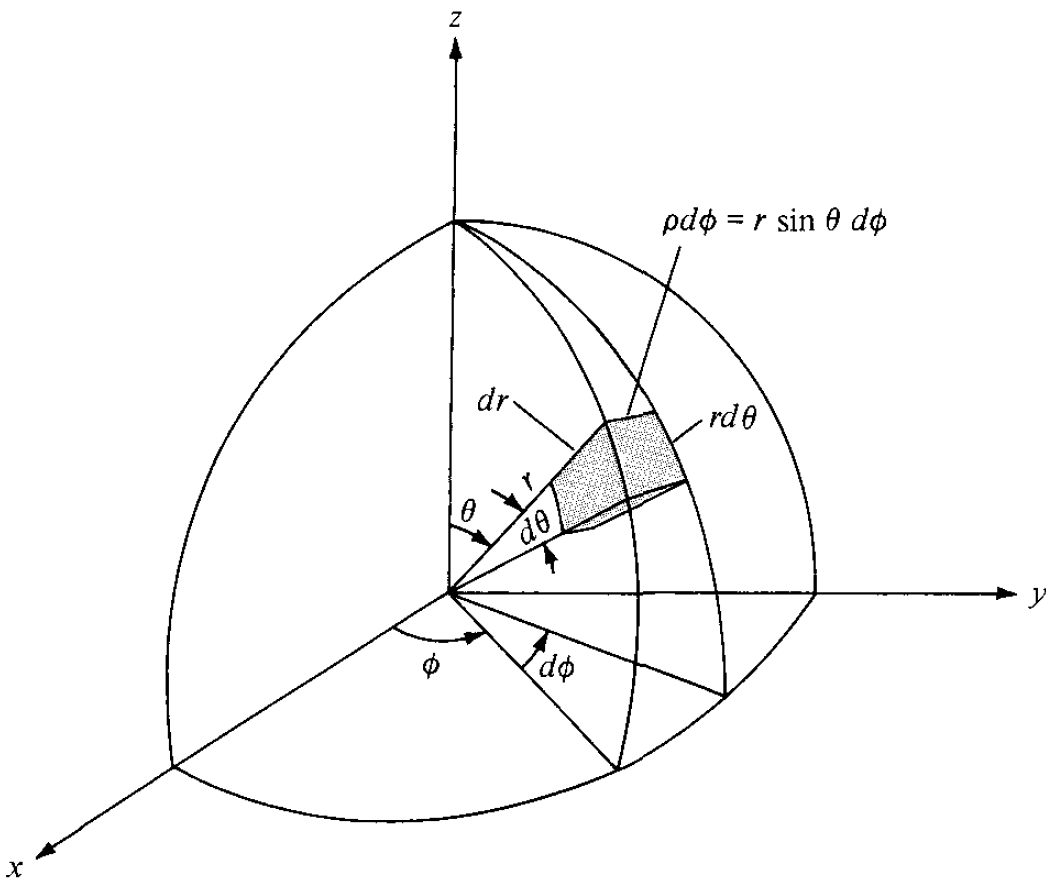
\includegraphics[scale=0.3]{Figure3-5S.png}
\caption{Differential volume in Spherical coordinates. Figure taken from~\cite[Figure 3.5, page 57]{Sadiku}}
\label{Spherical-differential-volume}
\end{figure}
\begin{figure}[h]
\centering
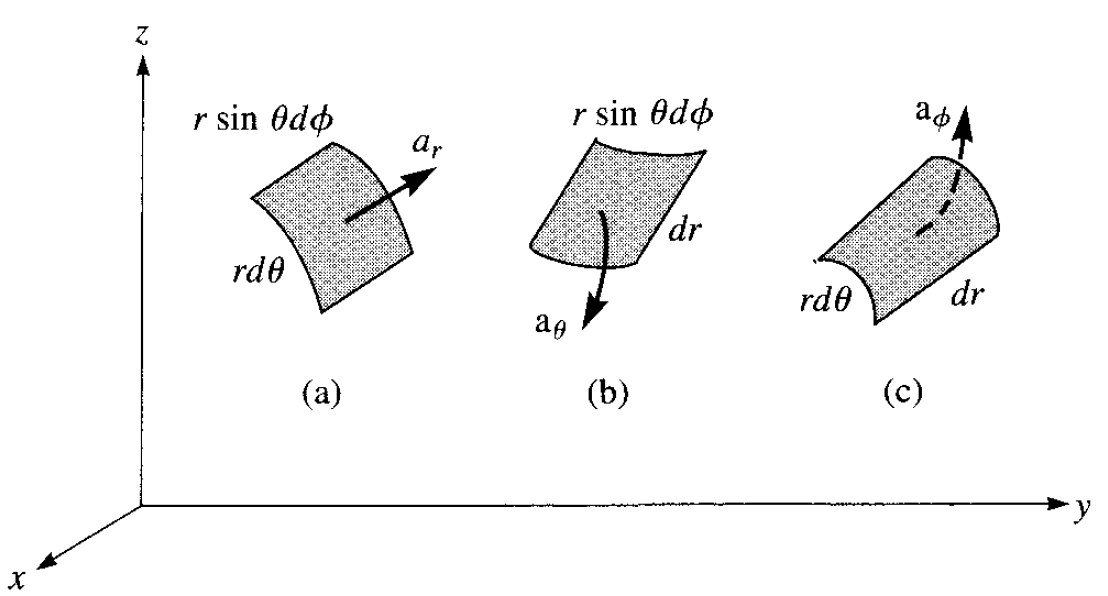
\includegraphics[scale=0.3]{Figure3-6S.png}
\caption{Differential normal areas in Spherical coordinates. Figure taken from~\cite[Figure 3.6, page 57]{Sadiku}}
\label{Spherical-differential-area}
\end{figure}
%\section{Introduction to the Line Integral}
%Line integral is the generalisation of single variable integral. You may have only seen integrals of the kind $\int_{x=a}^{x=b} f(x)dx$ till now. The path of this integration is along the $x$--axis from $x=a$ to $x=b$. In electromagnetics we come across integrals where the path of integration may be any arbitrary (curved or zig zag) path in 3D space. Two important line integrals are
%\begin{itemize}
%\item $\int_{a}^{b}\hat n\cdot d\textbf{\textit{l}}$~: Gives the length of the path from a to b if $\hat n$ is parallel to the path.
%\item $\int_{a}^{b}\textbf{A}\cdot d\textbf{\textit{l}}$~: If \textbf{A} is force, then this integral gives the total work done from a to b. If \textbf{A} is electric field then this integral gives potential difference (or voltage) between a and b.
%\end{itemize}
%Notice, these integrals give a scalar. There are other forms of line integrals but we will restrict ourselves to these two for now.
%\section{Using Calculator to Solve Integrals}
%A calculator can be used to solve definite integrals. To find $\int_{0}^{3}x^2dx$, the key sequence is: $\boxed{\int dx}$ $\boxed{ALPHA}$ $\boxed{X}$ \fbox{\textasciicircum} $\boxed{2}$ $\boxed{,}$ $\boxed{0}$ $\boxed{,}$ $\boxed{3}$ $\boxed{)}$ $\boxed{=}$. The answer should come out to be 9. The sequence of instructions is: integration notation followed by expression to integrate and then limits of integration. On newer models limits may be entered in boxes.
%
%It is important to note that the calculator only treats `X' as the variable of integration. So, if you need to evaluate $\int_{0}^{3}t^2dt$, the expression would be the same as above replacing t with `X' during input.
%\section{Exercises}
%\noindent\textbf{Question 1:} Using $\int_{a}^{b}\hat n\cdot d\textbf{\textit{l}}$
%\begin{itemize}
%\item[(1)] Find the length of line segment from (0, 0) to (1, 2). Solve this in Cartesian as well as Cylindrical coordinates.
%\item[(2)] Find the length of body/space diagonal of a unit cube.
%\item[(3)] Find the arc length of a quarter circle of radius $\rho=3$ m in first quadrant.
%\item[(4)] Find the length of the curve $y=x^2$ from (0, 0) to (1, 1). For this problem a calculator would be handy in solving the integrals.
%\end{itemize}
%\noindent\textbf{Note:} For part (4) you need to find a unit vector along the curve $y=x^2$. A vector parallel (or tangent) to $y=x^2$ can be obtained from the slope. Numerator and denominator of slope ($\dfrac{dy}{dx}$) are the $y$-- and $x$--components, respectively, of the vector. Here, $\dfrac{dy}{dx}=\dfrac{2x}{1}$ so the parallel/tangent vector is $\textbf{n}=\hat x+2x\hat y$. The unit vector is then $\hat n=\dfrac{\hat x+2x\hat y}{\sqrt{1+4x^2}}$.\\
%\noindent\textbf{Question 2 (Example 2--4C \cite[Example 2--4, page 23]{Cheng}):} Given a force field $\textbf{F}=xy\hat x+(3x-y^2)\hat y$ in a region, evaluate the integral $\int_{P1}^{P2}\textbf{F}\cdot d\textbf{\textit{l}}$ to find the total work done in moving from P1 to P2 along path 1 and path 2.\\
%\noindent\textbf{Question 3:} Electric field in a region is $\textbf{E}=x\hat x+y\hat y$. Refer to figure \ref{Cheng-integral}, evaluate the integral $\int_{P1}^{P2}\textbf{E}\cdot d\textbf{\textit{l}}$ to find the potential difference between P1 and P2. Is the potential difference same for path 1 and path 2?
%\begin{figure}[H]
%\centering
%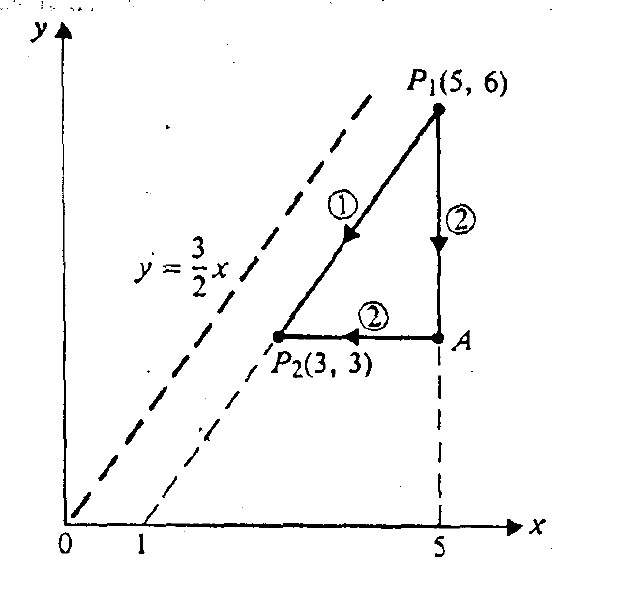
\includegraphics[scale=0.6]{Figure2-10Cheng.png}
%\caption{Paths of integration for Question 2 \cite[Figure 2--10, page 23]{Cheng}}
%\label{Cheng-integral}
%\end{figure}
%\nocite{*}
\bibliographystyle{plain}
\bibliography{PhysicsRef}
\end{document}
